% Chapter 2 is an English rendering of บทที่ 2 ทฤษฎี/งานวิจัยที่เกี่ยวข้อง in the
% faculty template (docs/MyThesisInfo/final_report.pdf, pp. 4-18).  The
% science is the template's; only the language changed.  Figure sources are
% carried over verbatim.
\chapter[THEORY AND RELATED WORK]{Theory and Related Work}
\label{chap:theory}

In carrying out the project ``Vision-Based Navigation Pipeline for AMRs in
Dynamic Warehouse'', the author's aim is to develop and evaluate only the
navigation pipeline, within the scope defined in \cref{sec:scope}. The project
does not set out to build a complete autonomous robot from scratch; it
integrates navigation software into the existing architecture of an autonomous
mobile robot (AMR). To make that development effective, the author studied and
collected theory, documents and research on the following principal topics.

\section{AMR Navigation Systems}
\label{sec:amr-navigation}

Autonomous mobile robots are among the technologies transforming industry in the
digital era, particularly in manufacturing, warehousing and materials handling.
With their capacity to learn, their flexibility and their high precision, AMRs
reduce cost and raise efficiency by a large step. This section reviews the
properties, technology and use cases of AMRs to make the potential of the
innovation clear.

\subsection{Logistics management and the historical bottleneck}

In a traditional warehouse, most wasted expenditure arises in the logistics of
moving material from one point to another, work that exhausts staff who must
walk while continuously carrying loads. These movements produce ``motion waste'',
one of the eight principal wastes of lean manufacturing
(\cref{fig:lean-wastes}). To stay competitive and cut logistics costs, smart
warehouses have begun to bring autonomous robots in to work alongside people
and reduce that time and waste.

\begin{figure}[htbp]
  \centering
  
\includegraphics[width=0.8\textwidth]{figures/template/lean_wastes.png}
  \caption[The eight principal wastes of lean manufacturing.]{The eight principal wastes of lean manufacturing. Source:
  \url{https://teachme-biz.com/th/blog/reduce-waste/}.}
  \label{fig:lean-wastes}
\end{figure}

\subsection{The era of automated guided vehicles (AGVs)}

Research and development of autonomous mobile robots began in the 1950s with
automated guided vehicles. AGV systems have an important limitation: the vehicle
depends on infrastructure installed in the warehouse beforehand for navigation,
such as magnetic tape, QR codes or artificial landmarks
(\cref{fig:agv-navigation}). AGVs can also only follow fixed, pre-planned
routes, so the system lacks spatial flexibility, and if the warehouse
environment changes the AGV cannot adapt immediately.

\begin{figure}[htbp]
  \centering
  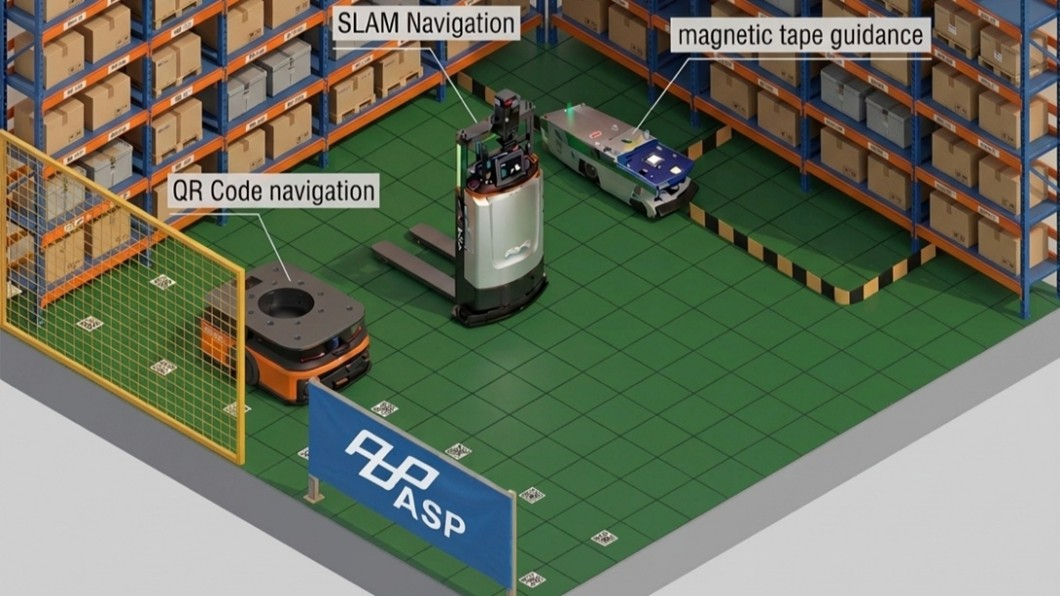
\includegraphics[width=0.8\textwidth]{figures/template/agv_navigation_types.jpg}
  \caption[Three warehouse robots with different navigation technologies: the orange robot uses QR-code navigation, the pallet truck in the centre uses SLAM navigation without floor infrastructure, and the white robot uses magnetic-tape guidance.]{Three warehouse robots with different navigation technologies: the
  orange robot uses QR-code navigation, the pallet truck in the centre uses SLAM
  navigation without floor infrastructure, and the white robot uses
  magnetic-tape guidance. Source:
  \url{https://www.linkedin.com/pulse/agv-amr-navigation-technologies-which-one-drives-your-abdul-rahman-6pjyc}.}
  \label{fig:agv-navigation}
\end{figure}

\subsection{The transition to autonomous mobile robots (AMRs)}

AMRs were developed to overcome the limitations of AGVs. The essential
difference is that an AMR can make its own decisions and does not need
pre-installed external infrastructure to navigate. Recent hardware advances,
particularly in imaging sensors (2-D/3-D cameras and LiDAR) together with
high-performance processors, let an AMR perceive and assess its surroundings
accurately. The distinguishing capability that lets AMRs replace AGVs is
operation in a dynamic environment: when an AMR detects an obstacle on its
route it can compute alternative routes to avoid the obstacle or another robot
automatically, without the user redesigning the route.

With this capacity for independent decision-making and navigation, large
industrial users have moved to AMRs widely. One example is the deployment of
autonomous driverless transport vehicles in the press plant of the BMW Group at
Regensburg~\cite{bmw2024}, whose vehicles navigate and manoeuvre precisely
through busy, complex areas of a real factory (\cref{fig:bmw-agv}), showing that
AMRs have fully overcome the limits of the older navigation systems.

\begin{figure}[htbp]
  \centering
  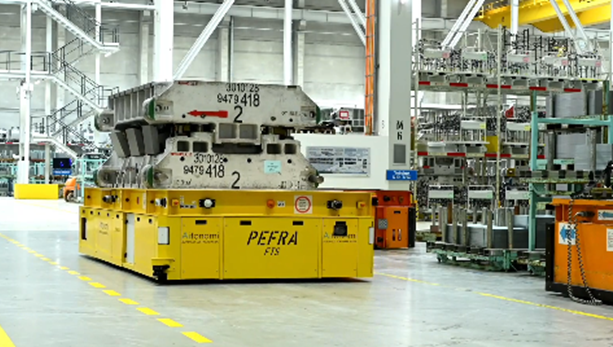
\includegraphics[width=0.7\textwidth]{figures/template/bmw_agv.png}
  \caption[An autonomous driverless transport vehicle navigating precisely in the BMW Group press plant at Regensburg.]{An autonomous driverless transport vehicle navigating precisely in
  the BMW Group press plant at Regensburg. Source:
  \url{https://www.press.bmwgroup.com/global/video/detail/PF0009726/}.}
  \label{fig:bmw-agv}
\end{figure}

\section{Visual Simultaneous Localization and Mapping (Visual SLAM)}
\label{sec:visual-slam}

In the operation of an AMR, localization is the heart of what lets the robot
move accurately. The widely accepted and used method is SLAM (simultaneous
localization and mapping). A SLAM navigation system extracts features present in
the environment to build a map; the software gathers information from the
robot's current position and the positions it has passed through to estimate a
probability distribution and predict the robot's most likely position.

\subsection{Components of a visual SLAM system}

This project concentrates on visual SLAM, mapping and localization with image
sensors, to reduce the cost of LiDAR sensors. Following the project's own
data-flow diagram, a visual SLAM architecture has three main parts
(\cref{fig:slam-indirect}):

\begin{enumerate}[leftmargin=2em]
  \item \textbf{SLAM front end (visual odometry)}: receives camera images and
    extracts features to estimate the robot's relative motion and pose over
    short intervals.
  \item \textbf{SLAM back end}: refines and corrects the accumulated drift of
    the front-end estimate using graph optimisation, to obtain the most accurate
    map and pose.
  \item \textbf{Loop closure}: the process by which the system recognises a
    place the robot has visited before; when the robot returns, the current
    image is matched to a past one and the whole map is corrected to reduce
    accumulated error.
\end{enumerate}

\begin{figure}[htbp]
  \centering
  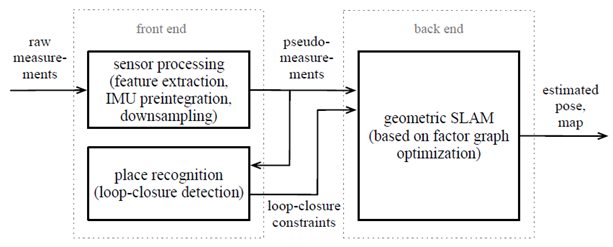
\includegraphics[width=0.85\textwidth]{figures/template/slam_indirect.png}
  \caption{The indirect (feature-based) method common to SLAM systems: a front
  end producing pseudo-measurements and loop-closure constraints, and a back end
  performing geometric SLAM by factor-graph optimisation~\cite{cadena2016}.}
  \label{fig:slam-indirect}
\end{figure}

\subsection{ORB-SLAM3}
\label{sec:theory-orb}

ORB-SLAM3~\cite{campos2021} is an open-source SLAM system that builds on the
success of ORB-SLAM and ORB-SLAM2. It is the first framework to support visual,
visual-inertial and multi-map SLAM with a range of camera types, monocular,
stereo and RGB-D, and with both pinhole and fisheye lens models
(\cref{fig:orbslam3-components}). The parts of its architecture and mechanisms
relevant to this project are as follows.

\begin{figure}[htbp]
  \centering
  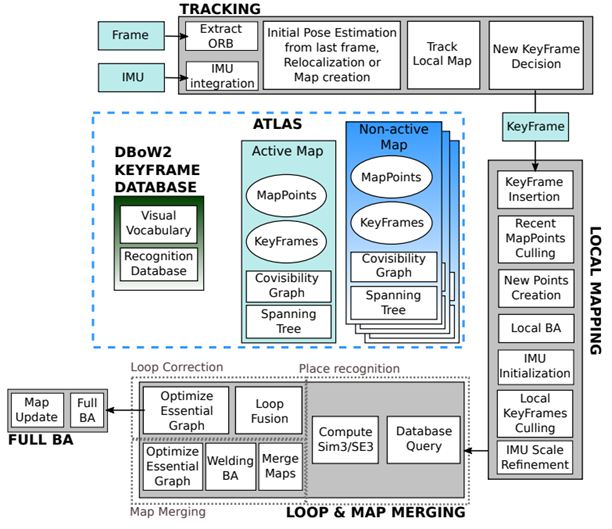
\includegraphics[width=0.8\textwidth]{figures/template/orbslam3_components.png}
  \caption{Main components of ORB-SLAM3: the tracking, local mapping and loop
  and map-merging threads around the Atlas multi-map representation and the
  DBoW2 keyframe database~\cite{campos2021}.}
  \label{fig:orbslam3-components}
\end{figure}

\subsubsection{Tightly-coupled visual-inertial SLAM}

One of the most important advances of ORB-SLAM3 is its visual-inertial SLAM
(VI-SLAM), which fuses data tightly by maximum-a-posteriori (MAP) estimation
both during initialisation and in normal operation, unlike earlier systems that
separated the computations. Its mechanisms are:

\begin{itemize}[leftmargin=2em]
  \item \textbf{Fast IMU initialisation.} The main problem of typical VI-SLAM
    systems is the delay in computing the IMU's initial parameters. ORB-SLAM3
    proposes a MAP uncertainty computation that recovers the map scale, the
    gravity direction and the gyroscope and accelerometer biases within about
    two seconds of start-up, so the robot obtains a correct pose with a
    physically true distance scale immediately.
  \item \textbf{Joint local bundle adjustment.} While moving, the system solves
    for the robot pose together with the 3-D landmarks and the IMU states
    (velocity and biases) simultaneously within a local window, compensating
    the accumulated drift of the images and the inertial sensor effectively.
\end{itemize}

\subsubsection{Atlas: multi-map system and place recognition}

To support lifelong mapping in an environment that changes or has visual
disturbances, such as a dynamic warehouse, ORB-SLAM3 introduces the Atlas map
management architecture, holding maps in two states:

\begin{itemize}[leftmargin=2em]
  \item \textbf{Active map}: the local sub-map the robot is currently using for
    tracking and mapping.
  \item \textbf{Non-active maps}: the set of past sub-maps the system has
    recorded and kept in memory.
\end{itemize}

When the robot passes through severe occlusion, or the lighting changes so far
that the camera cannot follow the previous features (tracking lost), an ordinary
SLAM system usually fails and stops. ORB-SLAM3 instead moves the map that lost
tracking into the non-active set and immediately starts a new active map to
continue localizing. When the robot later returns to a previously mapped area,
the place-recognition algorithm, with its improved recall, detects the overlap
and triggers map merging of the current active map with the earlier non-active
map, correcting the error by loop closure. This mechanism permanently reduces
the risk of the robot becoming lost in the warehouse.

\subsubsection{Abstract camera representation for wide-angle lenses}

Because this project selects the AC-IMX390-H190 camera with an ultra-wide
\SI{186}{\degree} field of view (fisheye lens), ORB-SLAM3 is technically well
suited: its architecture places an abstract representation layer between the
feature extractor and the camera projection model, so the system can switch to
the Kannala--Brandt fisheye model directly without affecting the back-end SLAM
algorithms. The robot can therefore process wide-angle images correctly and
without distortion in the localization result.

\subsection{VINS (Visual-Inertial System)}
\label{sec:theory-vins}

VINS (VINS-Mono, VINS-Fusion)~\cite{qin2018vins} is a high-performance
open-source state estimator developed by the Aerial Robotics Group (HKUST). Its
extended versions can fuse GPS, but for this project's indoor dynamic warehouse
VINS is used as a local 6-DoF visual-inertial odometry (VIO) estimator
(\cref{fig:vins-components}). Its main mechanisms are as follows.

\begin{figure}[htbp]
  \centering
  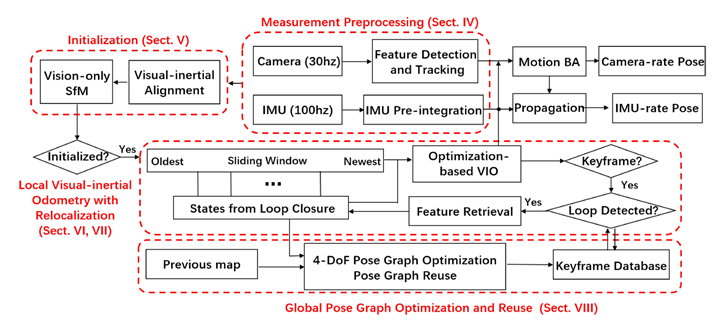
\includegraphics[width=0.95\textwidth]{figures/template/vins_components.png}
  \caption{Main components of monocular VINS: measurement preprocessing,
  initialisation, sliding-window visual-inertial odometry with relocalization,
  and global pose-graph optimisation and reuse~\cite{qin2018vins}.}
  \label{fig:vins-components}
\end{figure}

\subsubsection{IMU pre-integration}

In a fused sensor system the accelerometer and gyroscope deliver data at a very
high rate (\SIrange{100}{200}{\hertz}) while the camera delivers images at a
lower one (\SIrange{20}{30}{\hertz}). If a SLAM system re-integrated the IMU data
every time a pose was adjusted, the computational load would be enormous. VINS
solves this with IMU pre-integration: the accelerations and angular rates
between two consecutive image frames are integrated in the robot's local body
frame rather than the global frame, so the pre-integrated measurements do not
depend on the initial state and need not be recomputed when the back end
corrects the robot's pose. The system also propagates covariance and corrects
gyroscope and accelerometer bias through a first-order Taylor expansion, giving
a physically accurate pose estimate.

\subsubsection{Robust estimator initialisation}

A central challenge of visual-inertial SLAM is initialisation, because
monocular or stereo images carry no true metric scale at the outset and the IMU
carries accumulated bias. VINS establishes a tightly-coupled initialisation in
two steps:

\begin{itemize}[leftmargin=2em]
  \item \textbf{Local structure from motion (SfM).} Features are extracted and
    tracked over a window of time to build a 3-D structure and the relative
    camera poses first.
  \item \textbf{Visual-inertial alignment.} The SfM trajectory is set against
    the IMU pre-integration results to recover three initial quantities: the
    metric scale, the gravity direction relative to the robot, and the initial
    gyroscope bias. The AMR thereby perceives true metric distances in the
    warehouse immediately after it begins to move.
\end{itemize}

\subsubsection{Tightly-coupled sliding-window optimisation}

At the heart of the VINS pipeline is a sliding window that limits the number of
image frames and robot states that must be solved for. VINS forms a nonlinear
least-squares cost function, solved with Ceres Solver, in which three residuals
are tightly coupled:
\begin{equation}
  \min_{\chi}\Bigl\{\bigl\lVert r_p - H_p\chi\bigr\rVert^2
  + \sum_{k\in\mathcal{B}}\bigl\lVert r_{\mathcal{B}}\bigl(\hat{z}^{b_k}_{b_{k+1}},\chi\bigr)\bigr\rVert^2_{P^{b_k}_{b_{k+1}}}
  + \sum_{(l,j)\in\mathcal{C}}\bigl\lVert r_{\mathcal{C}}\bigl(\hat{z}^{c_j}_l,\chi\bigr)\bigr\rVert^2_{P^{c_j}_l}\Bigr\},
  \label{eq:vins-cost}
\end{equation}
where
\begin{itemize}[leftmargin=2em]
  \item the \textbf{marginalisation residual} $r_p$ is the prior obtained from
    past frames removed from the sliding window;
  \item the \textbf{IMU residual} $r_{\mathcal{B}}$ is the error between the
    robot's true state and the IMU pre-integration; and
  \item the \textbf{visual re-projection residual} $r_{\mathcal{C}}$ is the
    re-projection error of feature points on the stereo image plane.
\end{itemize}

\subsubsection{Marginalisation for real-time load control}

To keep the edge processor (NRU-51V) on the robot running in real time, VINS
removes frames from the sliding window under two conditions:

\begin{itemize}[leftmargin=2em]
  \item \textbf{Marginalise old (\texttt{MARGIN\_OLD}).} If the newest frame is
    judged a keyframe, the oldest frame in the window is removed, and its
    visual and inertial information is converted into a prior factor by the
    Schur complement so that important past parameters are not lost.
  \item \textbf{Marginalise second newest (\texttt{MARGIN\_SECOND\_NEW}).} If
    the newest frame is judged a non-keyframe (insufficient parallax), the
    second-newest frame is discarded outright without forming a prior. This
    bounds the density of the matrices and saves a great deal of computation
    when the AMR is stationary or moving slowly in the warehouse.
\end{itemize}

\subsubsection{Online temporal calibration}

A distinctive feature of VINS~\cite{qin2018td} is its treatment of temporal
misalignment between the camera and the IMU. In practice the camera trigger and
the IMU signals suffer transmission and triggering delays, so the two sensors'
timestamps disagree, an important cause of VIO failure when the robot moves fast
or turns. VINS adds the time offset as a state variable estimated jointly in the
back-end optimisation, computing the temporal shift of the image frames against
the IMU angular rate. The pipeline can thereby compensate the latency of the
AC-IMX390-H190 image stream on the processing board precisely, keeping tracking
consistent even when the robot vibrates on the \SI{5}{\degree} warehouse slope.

\subsection{RTAB-Map back end and memory management}
\label{sec:theory-rtab}

Following Labbé and Michaud~\cite{labbe2019}, RTAB-Map is an open-source SLAM
library designed to avoid failure through computational and memory explosion
when a robot operates over a large area or for a long time (lifelong mapping).
RTAB-Map receives odometry and point-cloud data from VINS and performs graph
SLAM in the back end through three main mechanisms
(\cref{fig:rtabmap-components}).

\begin{figure}[htbp]
  \centering
  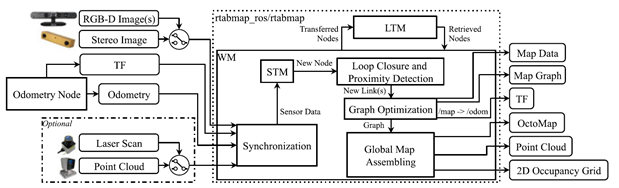
\includegraphics[width=0.95\textwidth]{figures/template/rtabmap_components.png}
  \caption{Main components of RTAB-Map: sensor synchronisation, short-term and
  working memory, long-term memory, loop-closure and proximity detection, graph
  optimisation and global map assembly~\cite{labbe2019}.}
  \label{fig:rtabmap-components}
\end{figure}

\subsubsection{Memory partitioning modelled on human memory}

RTAB-Map does not keep and compute over every map node in RAM; it organises the
data on three levels:

\begin{itemize}[leftmargin=2em]
  \item \textbf{Short-term memory (STM)} receives the latest image and odometry
    from VINS, extracts features and creates a new node. Nodes in STM are not
    yet used for loop-closure computation.
  \item \textbf{Working memory (WM)} is the main RAM area in which the
    algorithm detects loop closures and performs graph optimisation. The WM size
    is held constant by a time threshold so that the computation time never
    exceeds the real-time limit (for example \SI{<30}{\milli\second}).
  \item \textbf{Long-term memory (LTM)} is the database written to permanent
    storage (SSD or hard disk). Its contents do not enter the ordinary graph
    optimisation, conserving RAM and CPU.
\end{itemize}

\subsubsection{Memory transfer and weighting heuristics}

To lock the processing time at a constant ($O(1)$ time complexity) regardless
of how large the warehouse map becomes, RTAB-Map moves data between WM and LTM
as follows:

\begin{itemize}[leftmargin=2em]
  \item \textbf{Node weighting.} When the robot traverses a previous route and a
    loop closure occurs, the nodes there gain weight; frequently traversed nodes
    (such as the main warehouse aisles) carry high weight.
  \item \textbf{WM-to-LTM transfer.} When WM processing time approaches the set
    limit, the algorithm forces the ``oldest and least-weighted'' nodes out of
    RAM into LTM temporarily.
  \item \textbf{LTM-to-WM retrieval.} If the robot returns to an old area and
    feature extraction finds a link to a past node, the algorithm automatically
    retrieves the neighbouring nodes from LTM back into WM to connect the map
    structure and correct accumulated drift.
\end{itemize}

\subsubsection{Memory-constrained graph optimisation}

Unlike ordinary SLAM systems, which must optimise the graph over the whole map
and stall when run for a long time, RTAB-Map optimises the graph (through g2o or
GTSAM) only over the nodes remaining in working memory. The NRU-51V edge
processor can therefore run the navigation system and update the warehouse map
smoothly over its whole service life without loss of speed.

\section{Real-Time Object Detection}
\label{sec:object-detection}

\subsection{The role of object detection in semantic understanding}

In traditional geometric visual SLAM the algorithm extracts geometric features
without knowing what kind of object they belong to. For a warehouse that
changes continually, geometry alone is not enough: the system needs semantic
understanding to distinguish permanent structure from movable dynamic obstacles
(goods, pallets, people). This project therefore integrates object detection
into the front end to produce bounding boxes and pass the coordinates of dynamic
objects to the SLAM system, which masks out the unstable features.

\subsection{The YOLO (You Only Look Once) network architecture}

For the system to respond in real time while the SLAM system is running, the
project concentrates on the YOLO family, a one-stage detector distinguished by
its processing speed. Unlike two-stage models (such as Faster R-CNN) that first
generate region proposals and then classify them, YOLO predicts bounding-box
regression and class probabilities for the whole image in a single forward pass,
which makes YOLO (for example YOLO26) well suited to deployment on a
resource-limited edge processor such as the NRU-51V board.
\Cref{tab:detector-comparison} compares the main detector architectures.

\begin{table}[htbp]
\centering
\caption{Comparison of object-detection model architectures.}
\label{tab:detector-comparison}
\small
\setlength{\tabcolsep}{4pt}
\begin{tabularx}{\textwidth}{>{\raggedright\arraybackslash}p{0.14\textwidth}>{\raggedright\arraybackslash}p{0.13\textwidth}>{\raggedright\arraybackslash}X>{\raggedright\arraybackslash}X>{\raggedright\arraybackslash}p{0.18\textwidth}}
\toprule
Architecture & Category & Main strengths & Limitations & Suitable use \\
\midrule
Faster R-CNN & Two-stage detector & Excels in classification and localization,
  achieving high mAP and IoU with a low overall error rate and high spatial
  accuracy & The multi-stage process slows inference & Work requiring high
  accuracy without real-time processing \\
YOLO series & Single-stage detector & Casts detection as a single-stage
  regression problem tuned for speed, balancing speed and accuracy well, with
  high precision and recall and a low false-positive rate & Although now well
  refined, early versions had trouble with small or densely clustered objects
  compared with two-stage models & Real-time work requiring high processing
  speed and low latency \\
SSD (Single Shot Detector) & Single-stage detector & Removes the region-proposal
  step and performs multi-scale detection within one network & Sometimes
  slightly slower than YOLO, but still very efficient & Applications needing a
  reliable balance of throughput and accuracy \\
MobileNet / EfficientNet & Lightweight model & Uses techniques such as
  depthwise-separable convolutions to cut parameters and computation
  substantially without reducing learning capacity & Overall accuracy may be
  below large models such as Faster R-CNN or the larger YOLO versions & Edge
  devices with limited memory and compute: smartphones, IoT devices, drones \\
\bottomrule
\end{tabularx}
\end{table}

\subsection{Performance evaluation and edge-processor limits}

In bringing a YOLO model into a visual SLAM pipeline, the essential point is the
trade-off between accuracy and inference time (latency): too large a model
creates a bottleneck and makes the SLAM system fall behind the camera frame
rate. The evaluation of the YOLO model on a simulated warehouse dataset, through
a platform such as Roboflow, therefore uses the following main metrics:

\begin{itemize}[leftmargin=2em]
  \item \textbf{Intersection over union (IoU)}: the overlap ratio between the
    predicted box and the true object box, measuring localization accuracy.
  \item \textbf{Precision}: the fraction of dynamic-object predictions that are
    correct, out of all dynamic-object predictions (accuracy of the prediction).
  \item \textbf{Recall}: the fraction of dynamic objects correctly predicted, out
    of all dynamic objects actually present in the image (coverage of the
    search).
  \item \textbf{F1 score}: the harmonic mean of precision and recall, measuring
    the model's balance.
  \item \textbf{Average precision (AP) and mean average precision (mAP)}: the
    overall accuracy reflecting the model's combined performance across all
    object types under differing confidence thresholds.
\end{itemize}

Choosing the model with the highest mAP that still keeps latency within a safe
budget (for example \SIrange{<15}{20}{\milli\second}) is the key to a complete
integration of YOLO and SLAM.

\section{RY-SLAM: A Robust YOLO-Based Real-Time Visual SLAM Solution for
Dynamic Environments}
\label{sec:ryslam}

\subsection{Concept and architecture of RY-SLAM}

Chen et al.~\cite{chen2025} present RY-SLAM (Robust YOLO SLAM), an advanced
visual SLAM system designed to solve navigation failure in dynamic
environments. RY-SLAM integrates the ORB-SLAM3 framework with a YOLO-family
semantic detection and segmentation network (for example YOLOv8s-seg). Its
architecture relies on multi-threaded parallel processing with GPU
acceleration: the semantic-segmentation thread is separated from the SLAM
tracking thread, so the system can analyse dynamic-object coordinates and
estimate the camera pose at the same time without losing real-time throughput
(\cref{fig:ryslam-architecture}).

\begin{figure}[htbp]
  \centering
  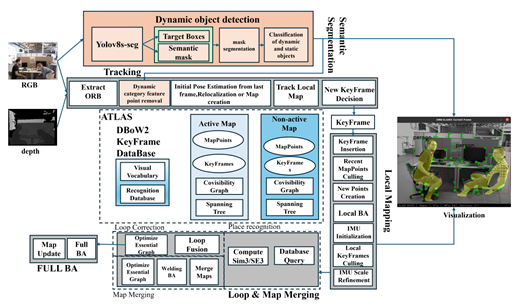
\includegraphics[width=0.9\textwidth]{figures/template/ryslam_architecture.png}
  \caption{Architecture of RY-SLAM: a YOLOv8-seg dynamic-object detection stage
  feeding a semantic mask into the ORB-SLAM3 tracking thread ahead of the Atlas
  multi-map system~\cite{chen2025}.}
  \label{fig:ryslam-architecture}
\end{figure}

\subsection{Dynamic feature masking mechanism}

The heart of RY-SLAM's localization accuracy is its dynamic feature masking,
in three technical steps:

\begin{itemize}[leftmargin=2em]
  \item \textbf{Semantic mask generation.} The YOLO model analyses the input
    frame to detect dynamic objects (such as people or vehicles) and generates
    a mask around each object's area.
  \item \textbf{Outlier elimination.} In the ORB-SLAM3 feature-extraction step
    the system checks the position of each ORB feature; any feature falling
    inside a dynamic-object mask is deleted immediately.
  \item \textbf{Static pose estimation.} Only features extracted from the
    permanent structure of the environment (static background) are fed to
    bundle adjustment, reducing accumulated drift and tracking loss
    significantly compared with standard ORB-SLAM3.
\end{itemize}

\begin{figure}[htbp]
  \centering
  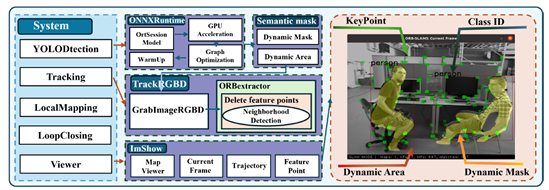
\includegraphics[width=0.9\textwidth]{figures/template/ryslam_framework.png}
  \caption[Detail of the semantic-segmentation framework in RY-SLAM and its multi-threaded operation: ONNX Runtime inference producing the dynamic mask, the neighbourhood test that deletes feature points, and the viewer outputs~\cite{chen2025}.]{Detail of the semantic-segmentation framework in RY-SLAM and its
  multi-threaded operation: ONNX Runtime inference producing the dynamic mask,
  the neighbourhood test that deletes feature points, and the viewer
  outputs~\cite{chen2025}.}
  \label{fig:ryslam-framework}
\end{figure}

\subsection{Relevance to this project}

RY-SLAM is important academic evidence for the effectiveness and soundness of
combining a YOLO-family model with ORB-SLAM3. For this project the author adopts
the basic concept and architecture of RY-SLAM and develops it further in
pipeline~1 (YOLO26 + ORB-SLAM3), raising system performance by choosing the
newer YOLO26 model to filter obstacles and mock goods in the warehouse in real
time, together with the Atlas multi-map architecture of ORB-SLAM3 on the NRU-51V
edge processor, so as to build a navigation system that is robust both to
close-proximity dynamic objects and in long-term (lifelong) mapping, as the
objectives require.
